\documentclass[xcolor={usenames}]{beamer}

\usepackage[spanish]{babel}
\usepackage[utf8]{inputenc}
\usepackage{multirow}

%formato de las diapositivas
\usetheme{Darmstadt}
\usecolortheme{rose}
\useoutertheme{shadow}
\useinnertheme{circles}

%colores
\definecolor{azul}{RGB}{0,0,255}
\definecolor{rojo}{RGB}{255,0,0}
\definecolor{verde}{RGB}{0,255,0}
\definecolor{naranja}{RGB}{255,175,0}
\definecolor{violeta}{RGB}{255,0,175}

%formato de la diapo de presentacion
\title[Informe final]{Placa de desarrollo}
\author[Carbonaro, Gomez, Spina]{C. Carbonaro \and F. Gómez \and J. Spina}
\institute[FIUBA]{
\begin{figure}
    \centering
    
\includegraphics[scale=0.1]{fiuba} 
\end{figure}
Universidad de Buenos Aires\\
Facultad de ingeniería}
\date{\today}
%Logo de la fiuba para todas las diapos
\pgfdeclareimage[height=1.2cm, width=1.2cm]{logo}{logo}
\logo{\pgfuseimage{logo}}

%\setbeamertemplate{navigation symbols}{} %quita los simbolos de navegacion

\begin{document}

\frame{\titlepage}
\section{Mediciones por generador}
\begin{frame}
\frametitle{Trabajo práctico grupal}

\begin{columns}[t]
		\column{0.5\textwidth}

Transceptor digital de sonido: consiste en un sistema capaz de digitalizar una señal de audio y transmitirla por medio de una interfaz UART. A la vez el sistema debe ser capaz de recibir datos digitales de audio, convertirlos a analógicos y reproducirlos por un parlante.
		
		\column{0.5\textwidth}
		\begin{figure}
			\centering
			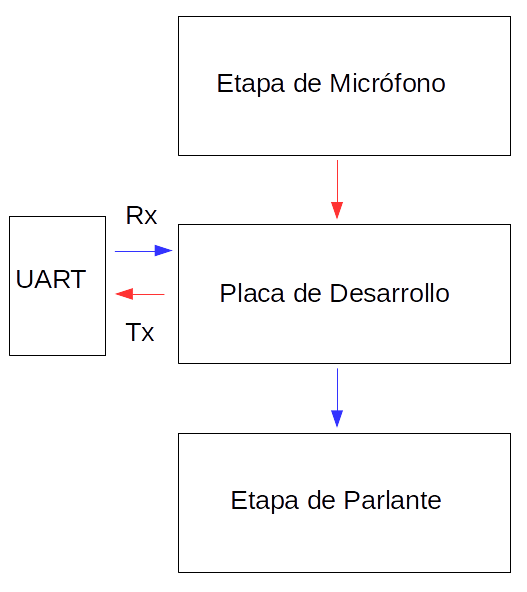
\includegraphics[scale=0.3]{diag1}	
		\end{figure}
	\end{columns}
\end{frame}

\begin{frame}
La etapa de micrófono consiste en un micrófono en si, un amplificador operacional (LM324) y un filtro RC de segundo orden.


\begin{columns}
    \begin{column}{0.5\textwidth}

     Se puede observar la deformación de la onda con un filtro de primer orden.

    \end{column}
    \begin{column}{0.5\textwidth}
      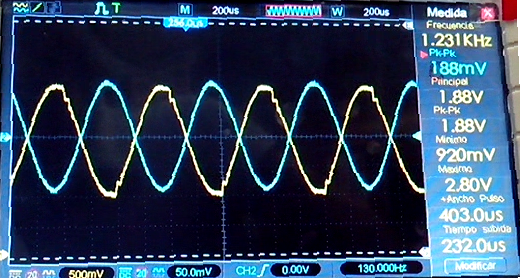
\includegraphics[width=.8\linewidth]{rcprimerorden}
    \end{column}
  \end{columns}

Con la implementación de un filtro de segundo orden se logró evitar estas deformaciones en la salida, así como también una mejor atenuación de la respuesta en frecuencia, conservando los niveles de ganancia (debido al seguidor de tensión).
\end{frame}


\begin{frame}

La placa de desarrollo se utiliza en tres facetas importantes
\begin{itemize}

\item Transmisión y recepción via UART: Establece la comunicación con otro transceptor.

\item Conversor analógico-digital: la señal que se recibe de la etapa de micrófono se muestra al doble de frecuencia de corte del filtro anterior inmediato.

\item PWM: Al recibir una señal digital del exterior, se recrea la señal analógica mediante la modificación del ancho de pulso PWM, mediante el valor medio de la señal. A la salida se coloca un filtro RC para no trabajar con frecuencias inutiles.


\end{itemize}

La etapa de parlante consiste en un amplificador de potencia y un parlante en si.

\end{frame}
\section{Vista general}
\begin{frame}
\frametitle{Vista general}
\begin{columns}[t]
\column{0.7\textwidth}
\begin{figure}
\centering
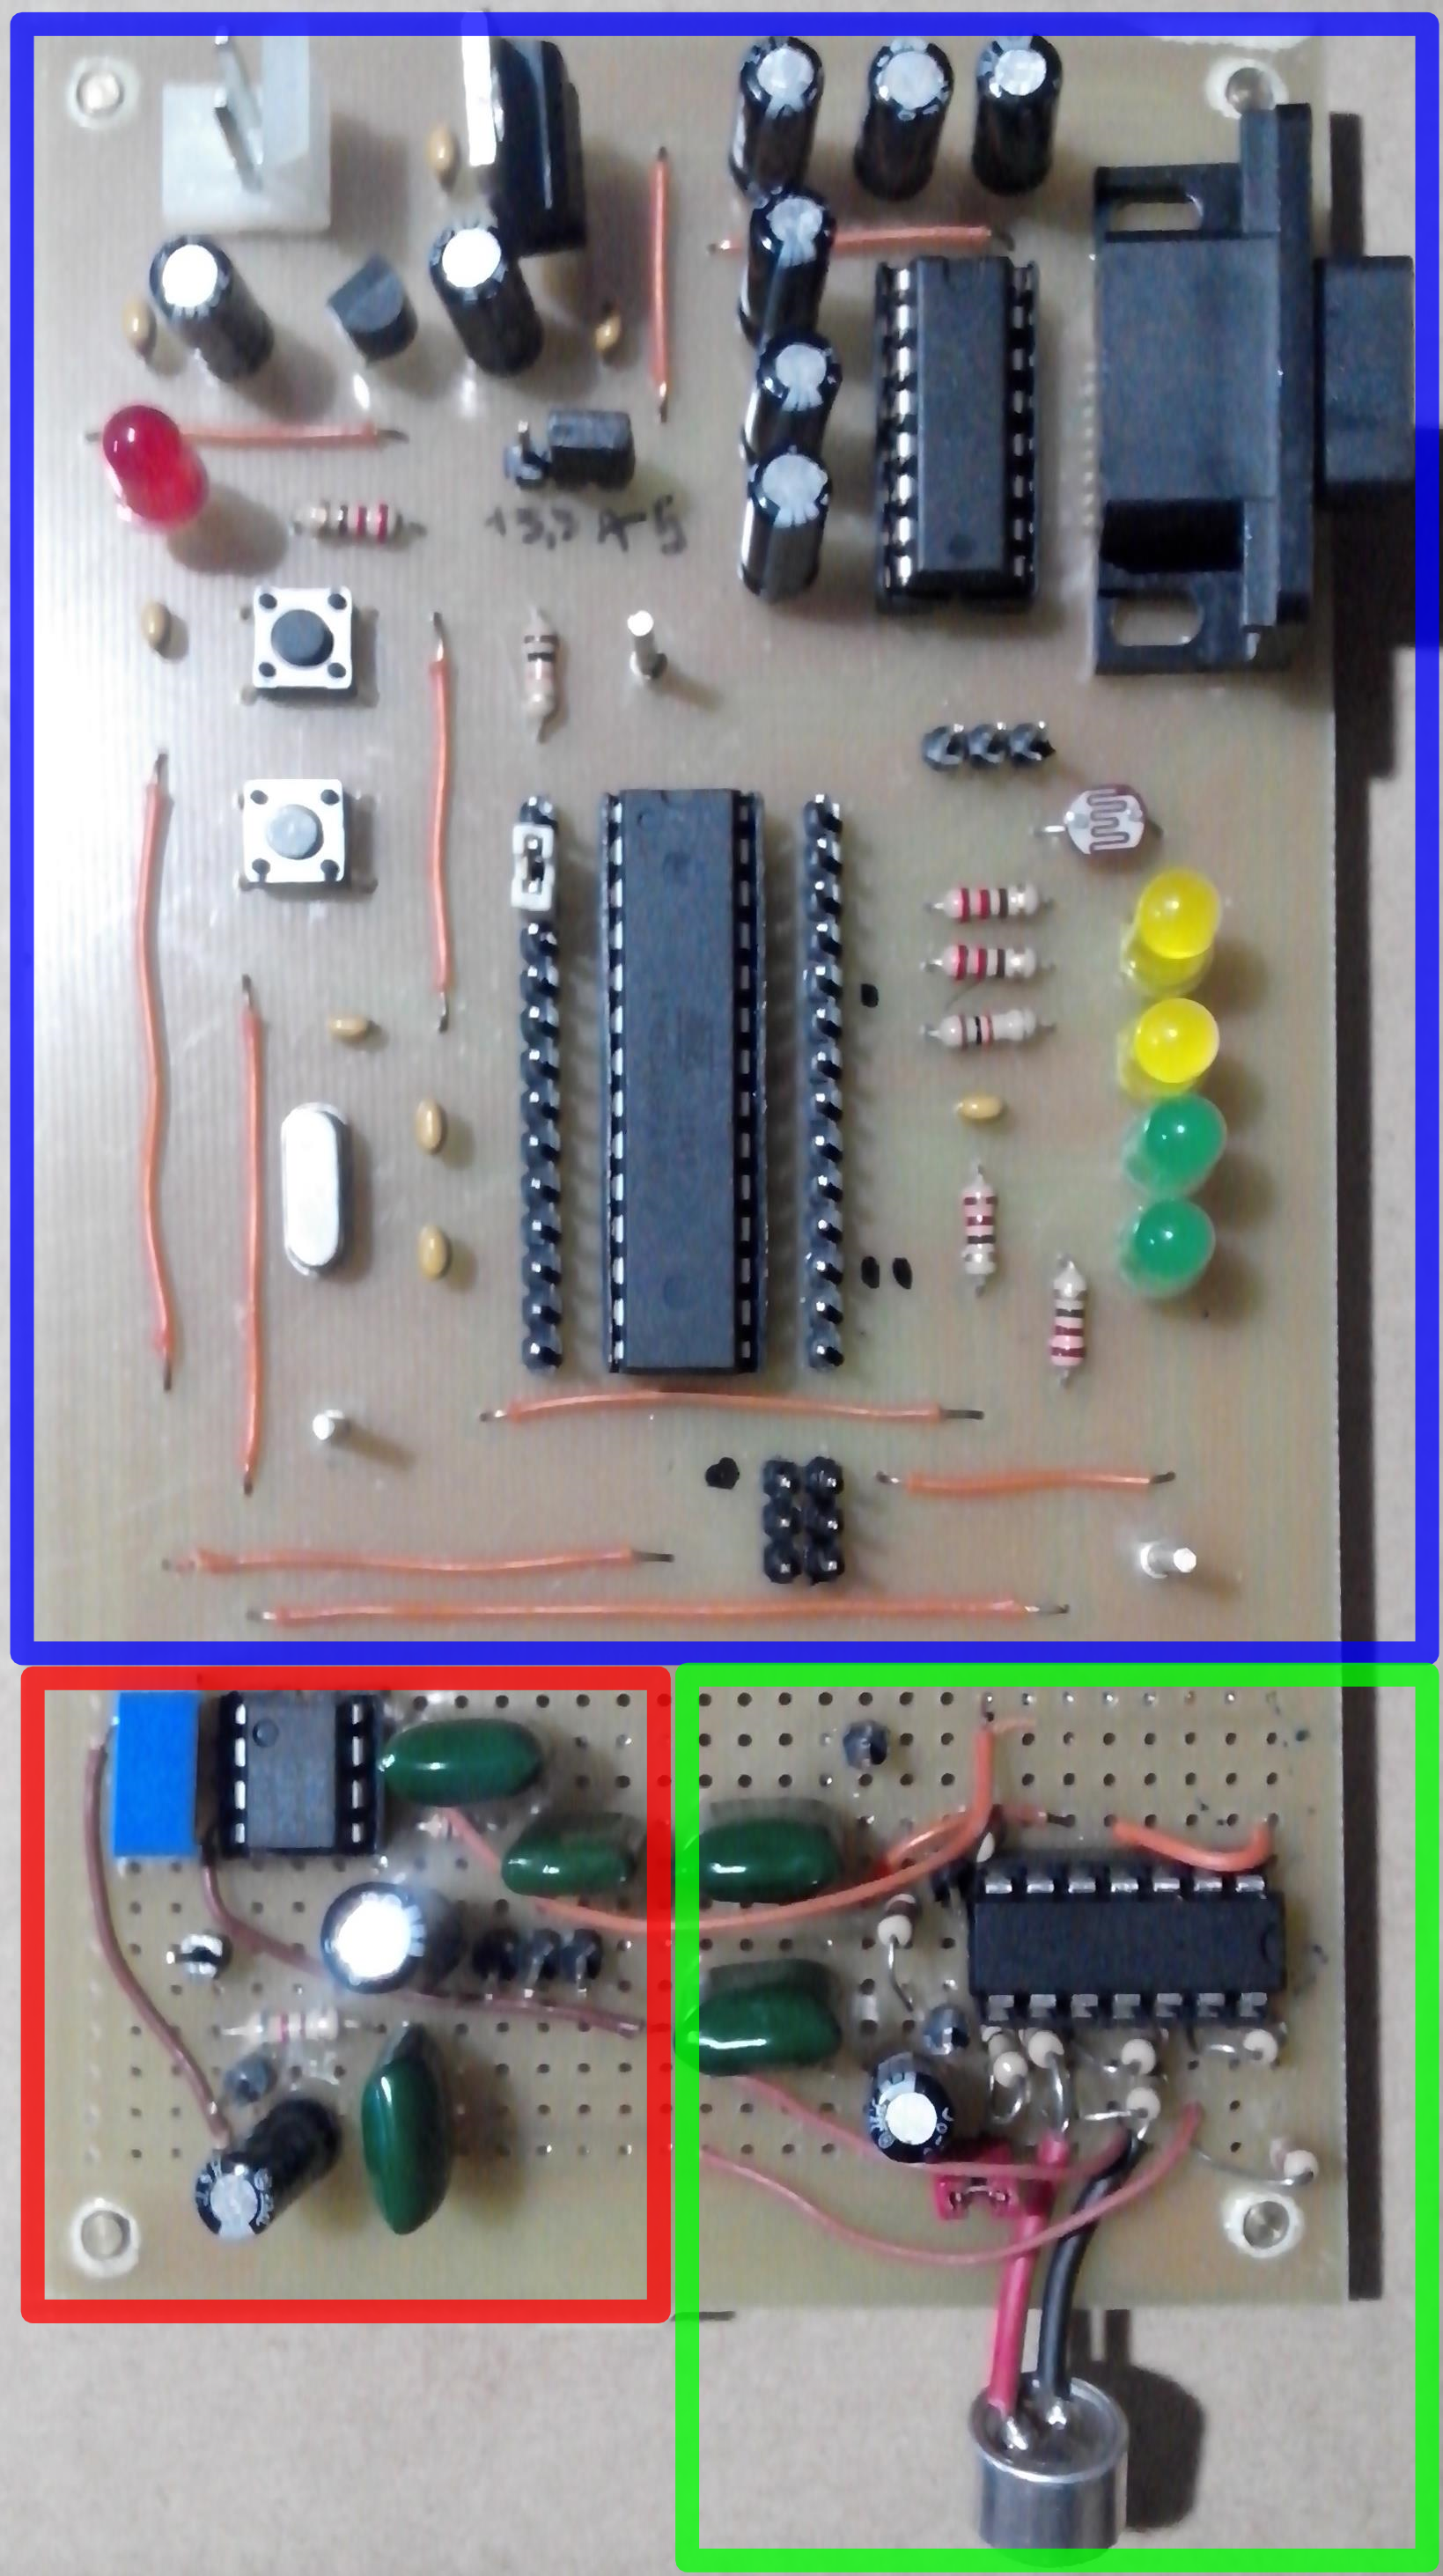
\includegraphics[scale=.08]{Placa}
\end{figure}
\column{0.3\textwidth}


\textcolor{azul}{Microcontrolador}

\textcolor{rojo}{Amplificador para parlante}

\textcolor{verde}{Amplificador para micrófono}
\end{columns}
\end{frame}

\begin{frame}
\frametitle{Vista general cont.}
\begin{columns}
\column{0.7\textwidth}
\begin{figure}
\centering
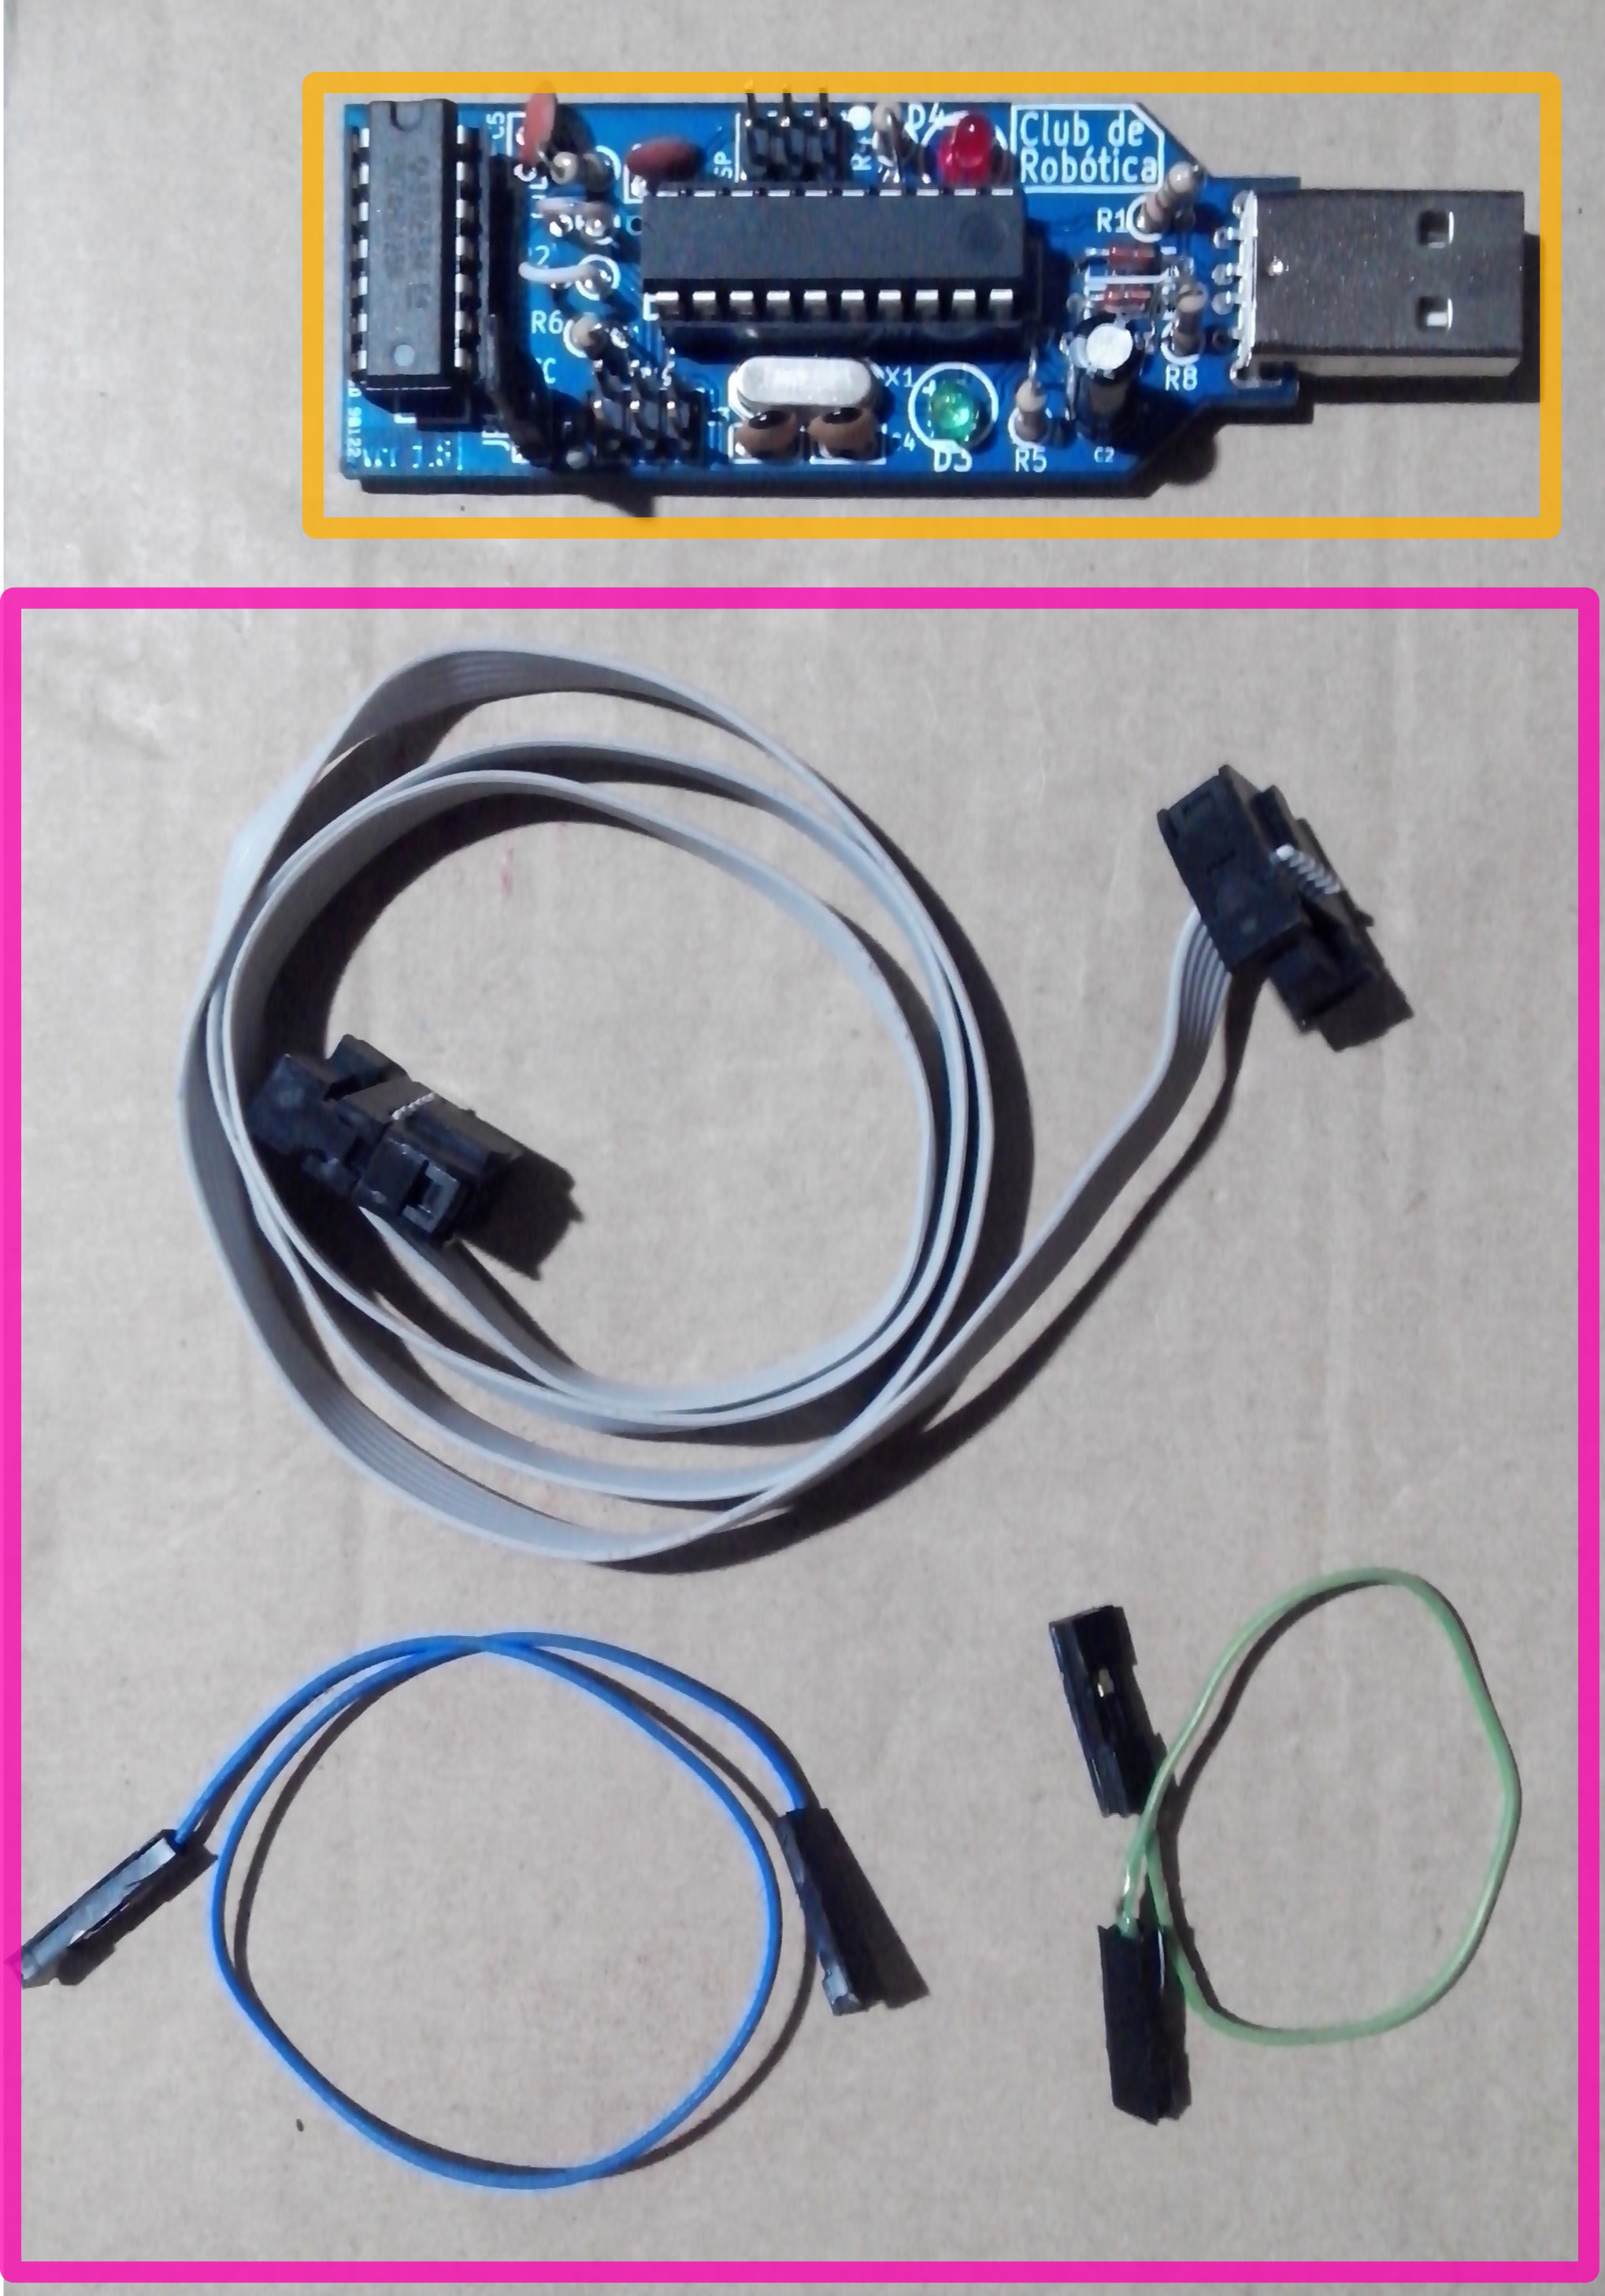
\includegraphics[scale=.09]{programador}
\end{figure}
\column{0.3\textwidth}
\textcolor{naranja}{Programador}

\textcolor{violeta}{Conectores}
\end{columns}
\end{frame}
\section{Microcontrolador}
\begin{frame}
\frametitle{Microcontrolador}
\begin{figure}
\centering
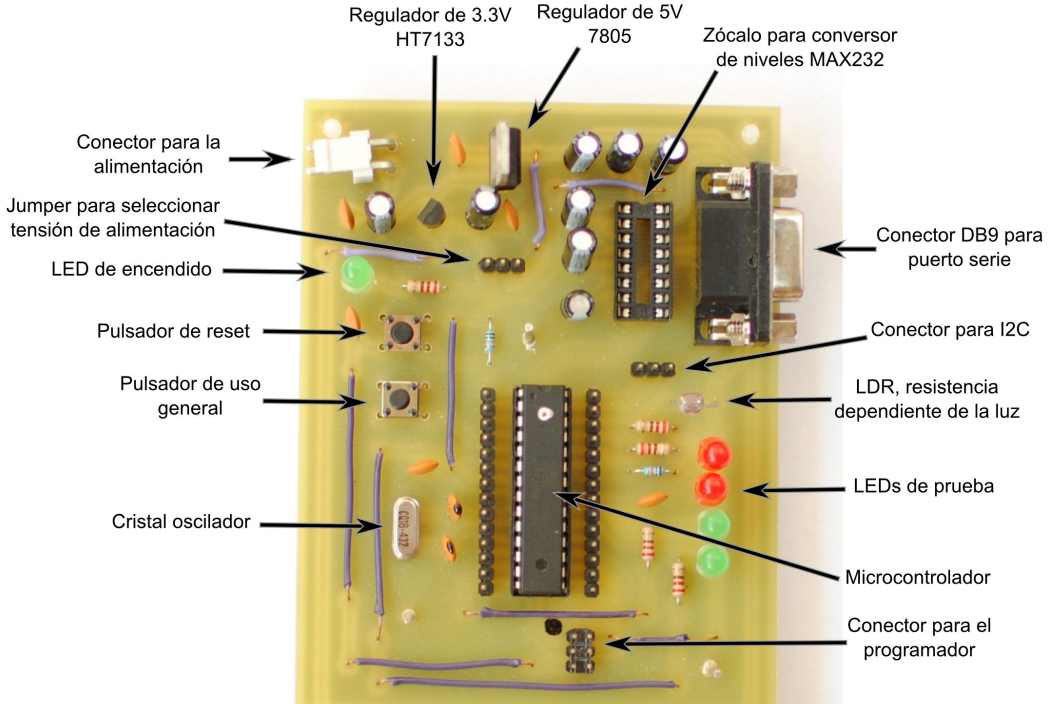
\includegraphics[scale=0.4]{PlacaDescrip}
\end{figure}
\end{frame}
\section{Medicion en continua}
\begin{frame}
	\frametitle{Mediciones en continua: Microfono}
	\begin{columns}[t]
		\column{0.6\textwidth}
		\begin{figure}[H]
			\centering
			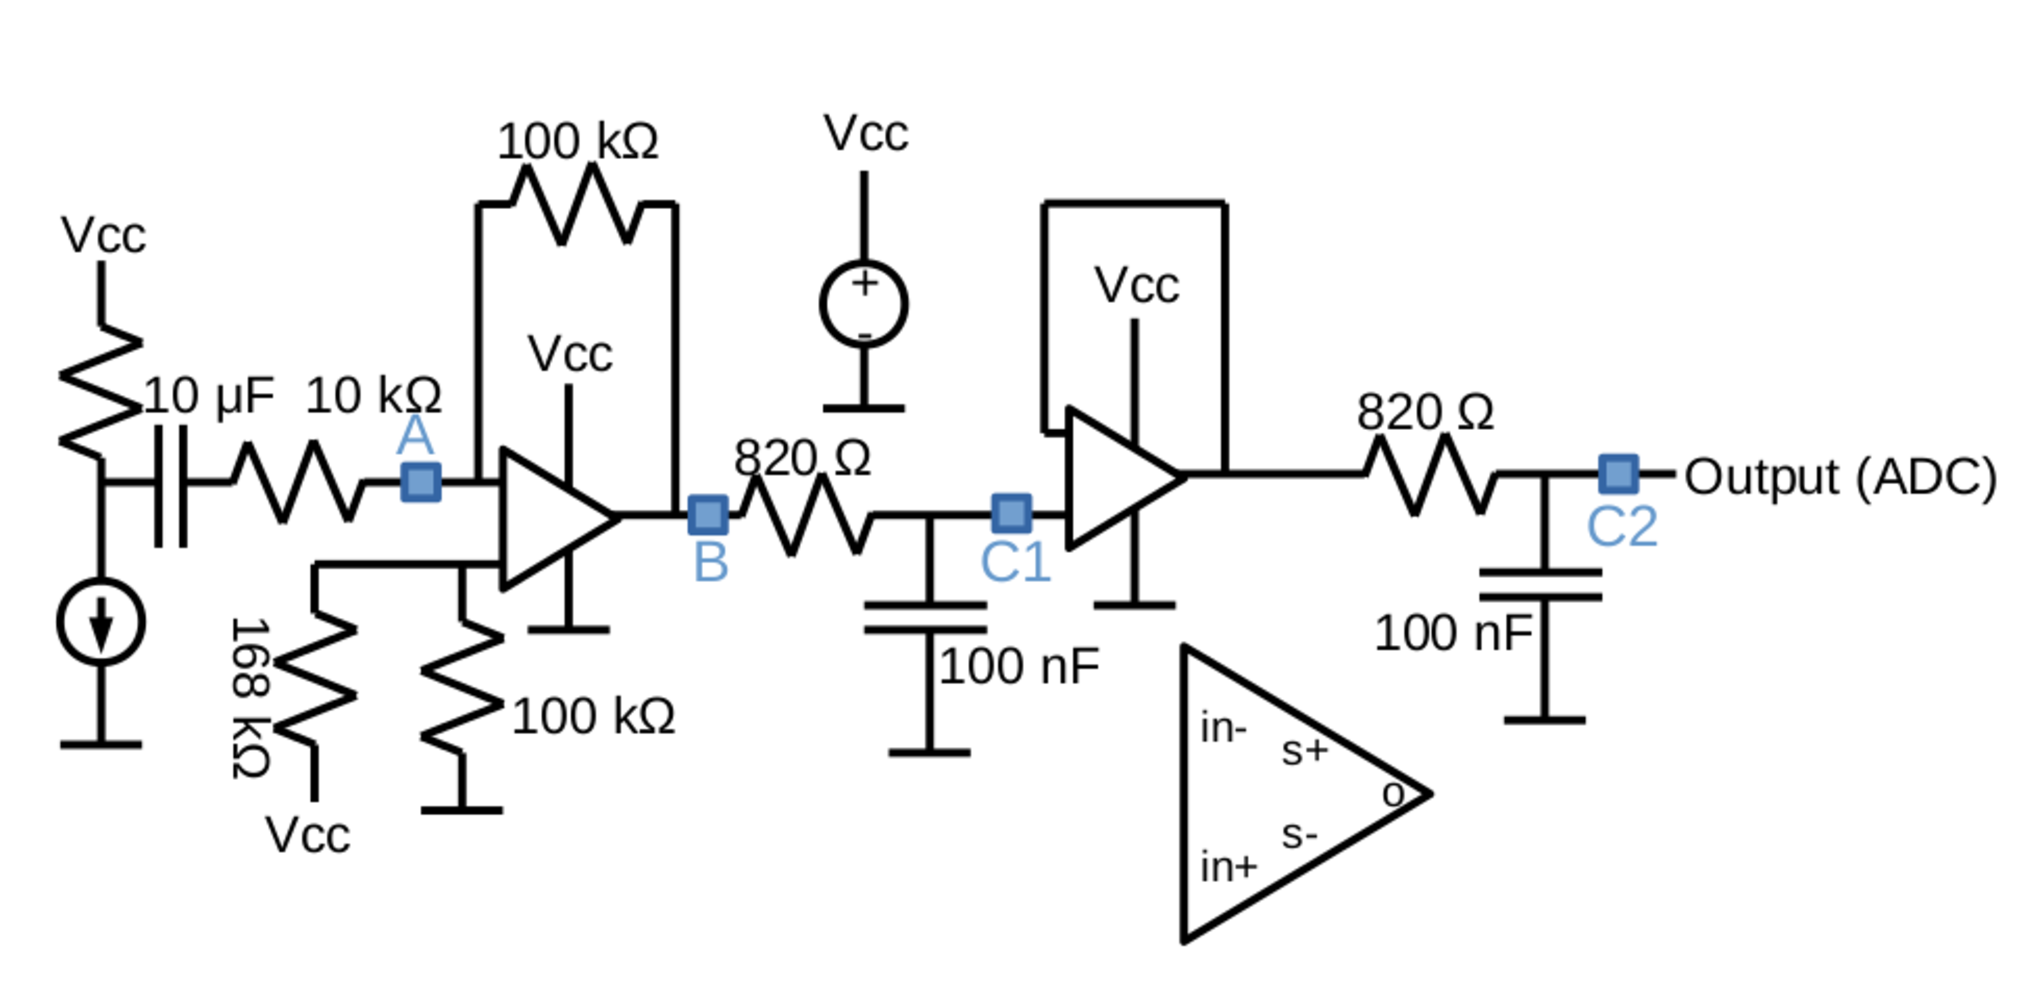
\includegraphics[scale=0.3]{AmpMic}	
		\end{figure}
		\column{0.4\textwidth}
		\begin{table}
			\centering
			\begin{tabular}{c|c}
				Punto & Tensión\\
				\hline \hline
				A & $(1.86;0.02)V$  \\
				\hline
				B & $(1.88;0.02)V$\\
				\hline
				C1 & $(1.87;0.02)V$\\
				\hline
				C2 & $(1.88;0.02)V$\\
				\hline
			\end{tabular}
		\end{table}
	\end{columns}
\end{frame}

\begin{frame}
\frametitle{Mediciones en continua: Microcontrolador}
	\begin{columns}[t]
		\column{0.6\textwidth}
		\begin{figure}
			\centering
			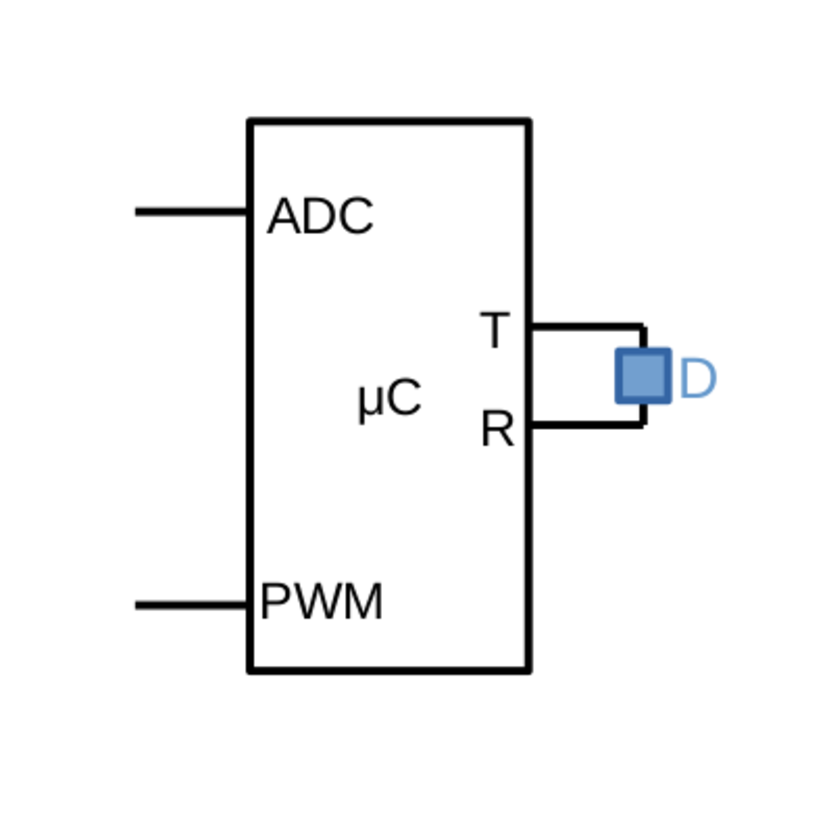
\includegraphics[scale=0.4]{MicroCon}	
		\end{figure}
		\column{0.4\textwidth}
		\begin{table}
			\centering
			\begin{tabular}{c|c}
				Punto & Tensión\\
				\hline \hline
				D & $(1.87;0.02)V$  \\
				\hline
			\end{tabular}
		\end{table}
	\end{columns}
\end{frame}

\begin{frame}
\frametitle{Mediciones en continua: Parlante}
	\begin{columns}[t]
		\column{0.6\textwidth}
		\begin{figure}
			\centering
			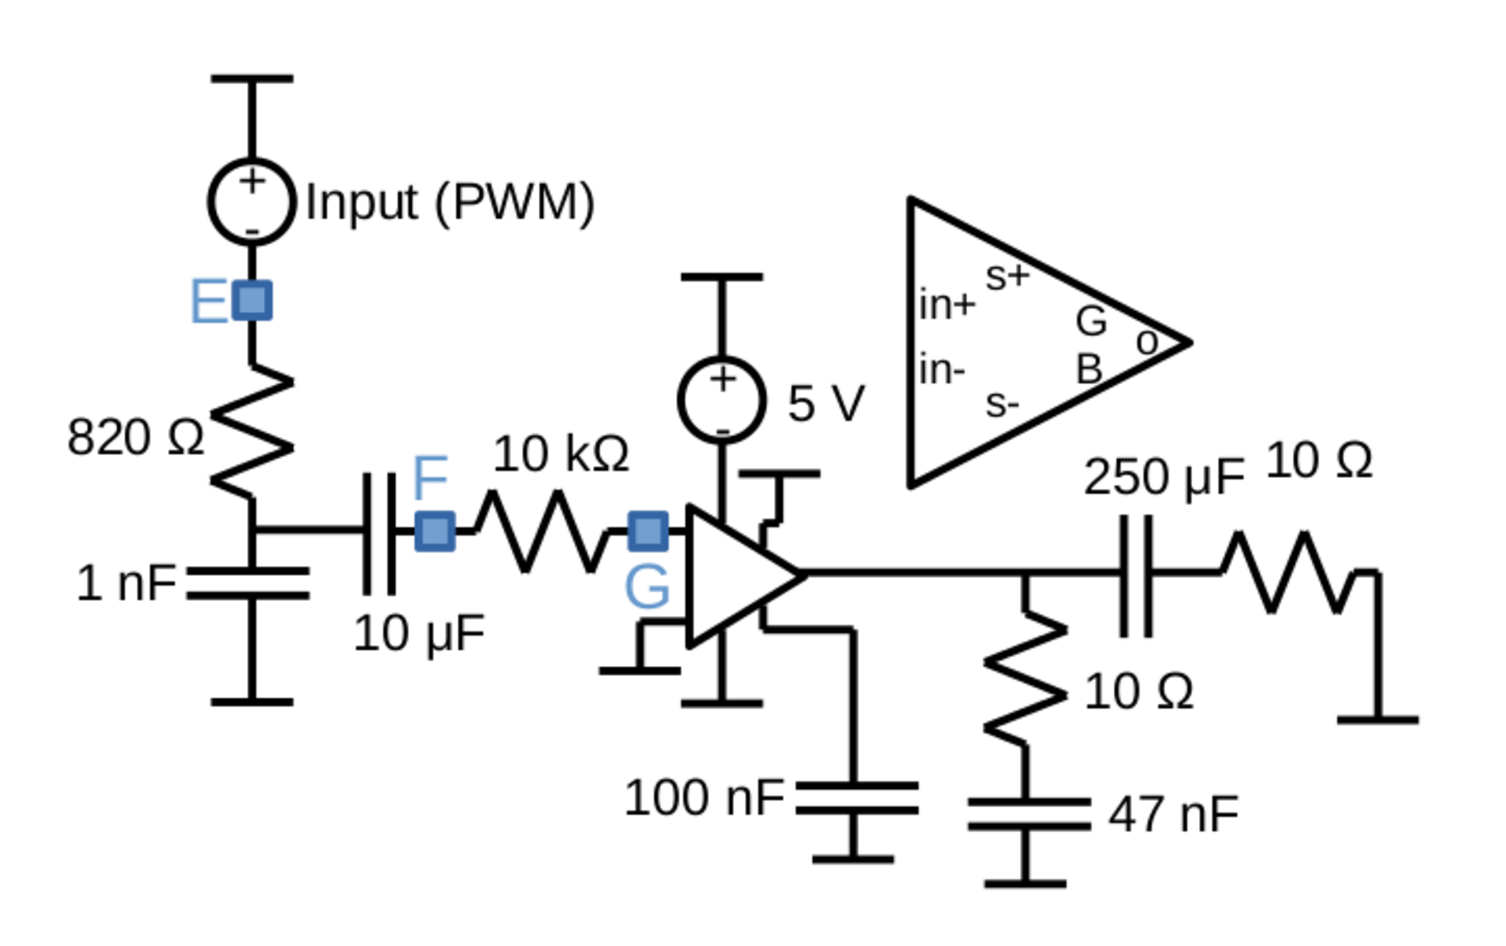
\includegraphics[scale=0.3]{AmpPar}	
		\end{figure}
		\column{0.4\textwidth}
		\begin{table}
			\centering
			\begin{tabular}{c|c}
				Punto & Tensión\\
				\hline \hline
				E & $(1.88;0.02)V$  \\
				\hline
				F & $(1.87;0.02)V$\\
				\hline
				G & $(0.000;0.002)V$\\
				\hline
				H & $(0.000;0.002)V$\\
				\hline
			\end{tabular}
		\end{table}
	\end{columns}
\end{frame}
\section{Mediciones por generador}
\begin{frame}
	\frametitle{Mediciones en Alterna}
	\begin{columns}[t]
		\column{0.6\textwidth}
		\begin{figure}
			\centering
			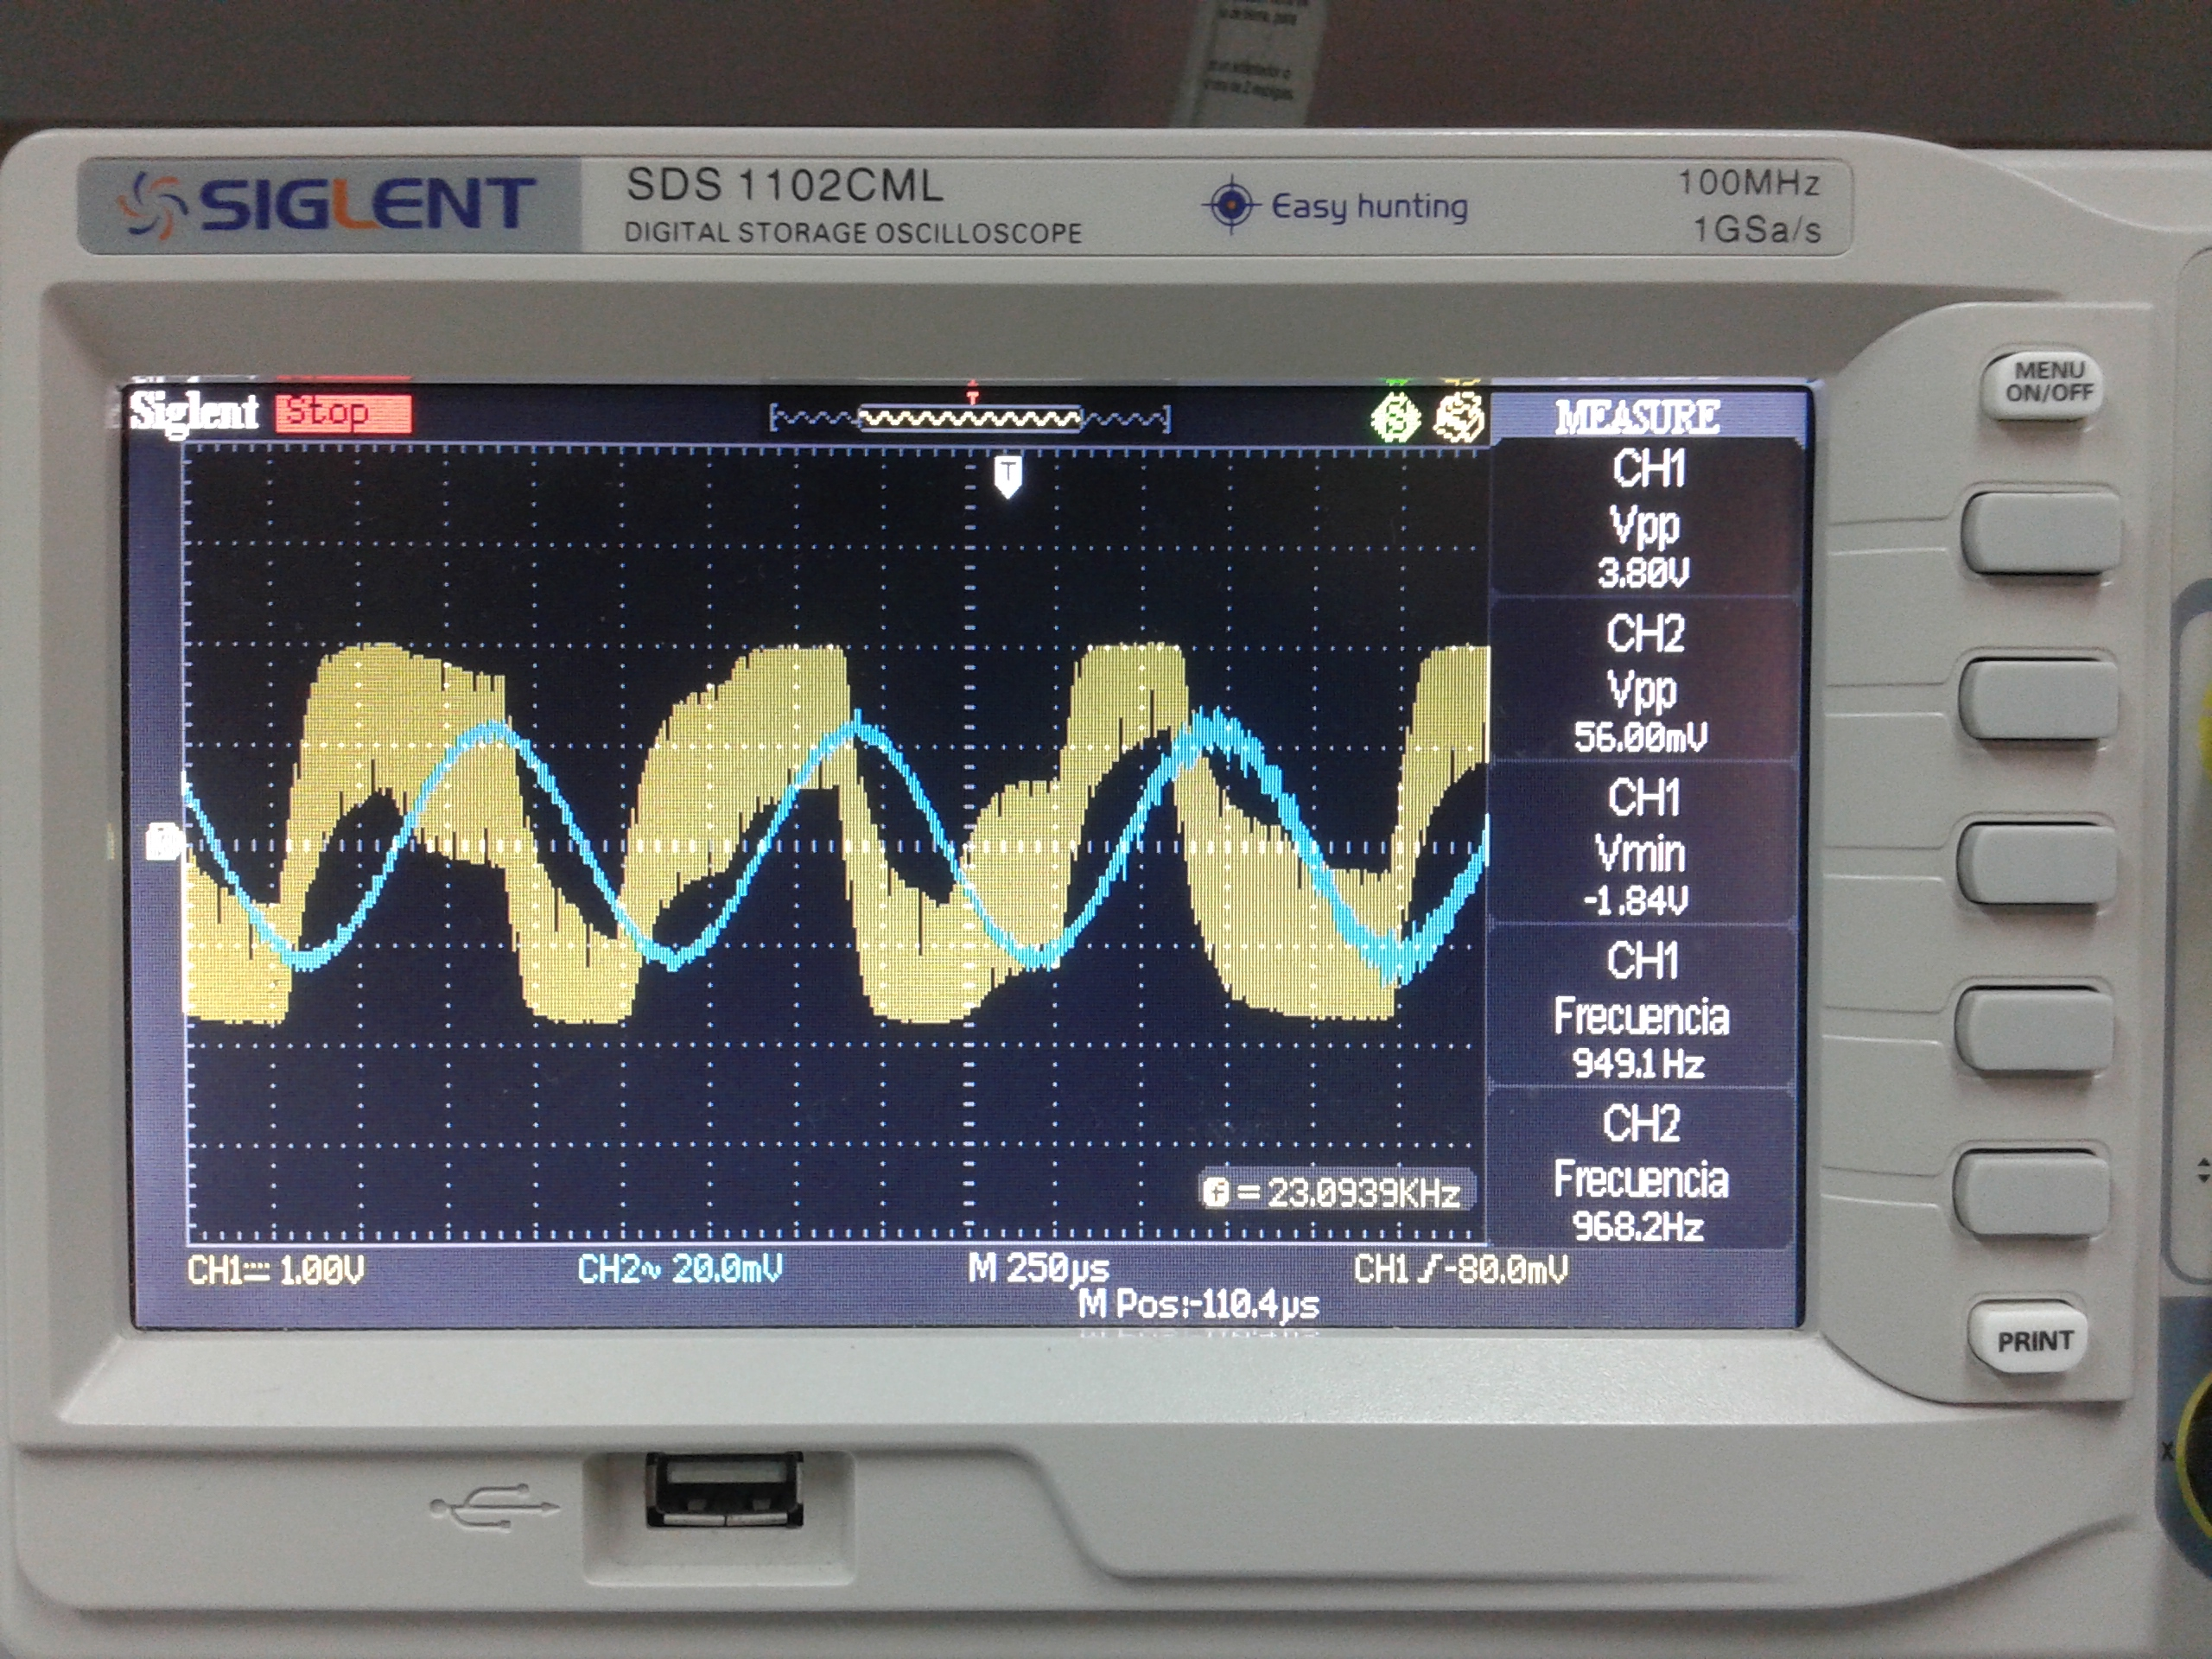
\includegraphics[scale=0.05]{20141201_152841}
           \caption{Comparación: entrada del generador vs salida al parlante}
		\end{figure}
		\column{0.4\textwidth}
		\begin{table}
			\centering
			\begin{tabular}{c|c}
				Punto & Vpp \\
				\hline \hline
				A & $(180;10)\>mV$   \\
				\hline
				B & $(1,6;0,2)\>V$ \\
				\hline
				C1 & $(1,4;0,2)\>V$ \\
				\hline
				C2 & $(1,3;0,2)\>V$ \\
				\hline
				D & $(4,8;0,2)\>V$  \\
				\hline
				E & $(5,1;0,2)\>V$ \\
				\hline
				F & $(520;10)\>mV$ \\
				\hline
				G & $(310;10)\>mV$ \\
				\hline
				H & $(2,7;0,1)\>V$ \\
				\hline
				\end{tabular}
		\end{table}
	\end{columns}
\end{frame}
\section{Microfono: implementación de filtro de segundo orden}
\begin{frame}
\frametitle{Filtro de segundo orden en el micrófono}
Se decidió implementar un filtro de segundo orden para lograr una mejor atenuación de la onda a frecuencias cercanas a los $2kHz$.
\begin{figure}[H]
			\centering
			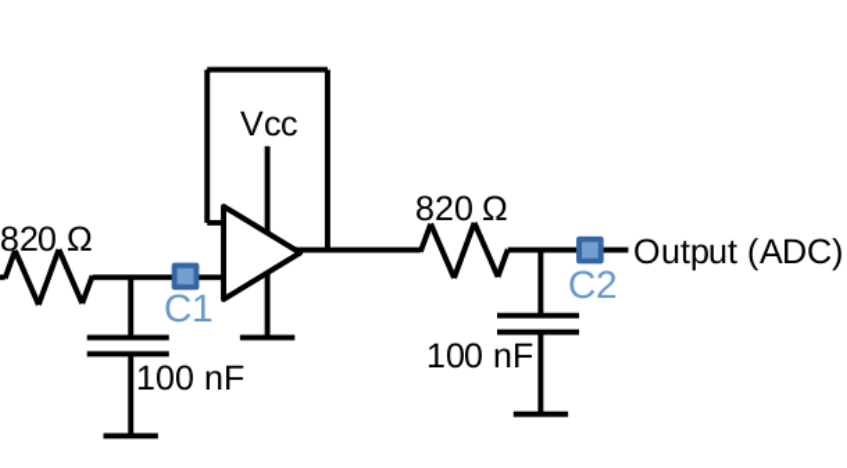
\includegraphics[scale=0.3]{esqfiltro}
			\caption{Esquema del filtro implementado en la salida del micrófono}	
		\end{figure}
\end{frame}



\begin{frame}
\frametitle{Filtro de segundo orden:Gráfico}
\begin{columns}[t]
		\column{0.5\textwidth}
		\begin{figure}[H]
			\centering
			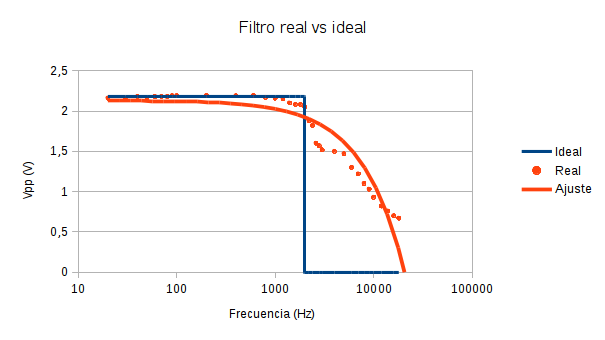
\includegraphics[scale=0.3]{Graf}
			\caption{Gráfico de la respuesta de tensión en función de la frecuencia para un filtro de \emph{primer} orden}	
		\end{figure}
		\column{0.5\textwidth}
		\begin{figure}[H]
			\centering
			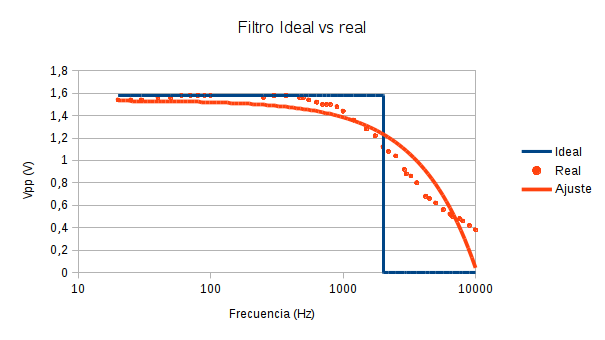
\includegraphics[scale=0.3]{Graf2do}
			\caption{Gráfico de la respuesta de tensión en función de la frecuencia para un filtro de \emph{segundo} orden}	
		\end{figure}
	\end{columns}
2\end{frame}
\end{document}